\chapter{Modelagem}

O presente trabalho resolve o problema da maior subsequência comum à 
duas palavras \emph{(LCS)} apresentando três soluções. Cada solução 
engloba um paradigma de programação.

A primeira solução apresenta uma abordagem \emph{força bruta} Ótima. A 
segunda utiliza o paradigma \emph{guloso} e discute a otimalidade da 
solução. A terceira apresenta um algorítmo Ótimo utilizando 
\emph{programação dinâmica} e discorre sobre sua \emph{subestrutura 
ótima} e \emph{sobreposição de subproblemas}, além de apresentar a 
\emph{equação de recorrência} em que o algorítmo é baseado.

\section{Metodologia}


\section{Solução}

\subsection{Força Bruta}

Em uma abordagem \emph{força bruta} para resolver o \emph{LCS} deve-se
enumerar todas as subsequências de uma palavra $X$ e verificar se cada
subsequência é comum a outra palavra $Y$. Com isso recuperar a maior 
subsequência comum às duas palavras. 

Dada uma palavra $X$ de tamanho n, tem-se que o número de
subsequência possíveis em $X$ pode ser representado por $2^n$. Essa 
abordagem requer um custo de tempo exponencial para chegar a solução, 
logo, impraticável para sequências muito longas. Para encontrar todas
as combinações (subsequências) foi utilizado um critério de caminhamento
sistemático em uma \emph{árvore de recursão}. Para compreender a 
estratégia, suponha uma palavra $X = abc$ cuja a \emph{árvore de 
recursão} pode ser vista na figura \ref{fig:recursiontree}.

\begin{figure}
\begin{center}
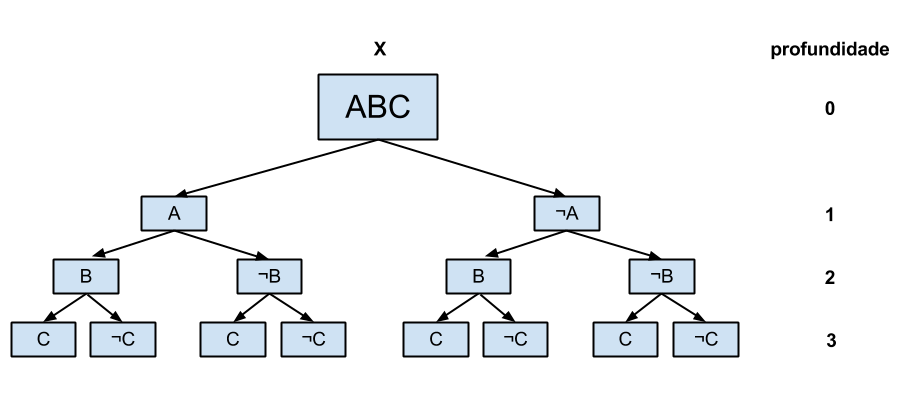
\includegraphics[width=0.8\textwidth,natwidth=610,natheight=642]{doc/recursion-tree.png}
\caption{Árvore de Recursão}
\label{fig:recursiontree}
\end{center}
\end{figure}


\subsection{Guloso}


\subsection{Programação Dinâmica}
